\documentclass[a4paper,11pt]{article}

\usepackage[utf8]{inputenc}

\usepackage{graphicx}
\usepackage{caption}
\usepackage{subcaption}

\usepackage{pgfplots}
\usepackage{float}
\usepackage{hyperref}
\usepackage{soul}
\hypersetup{
    colorlinks=true, % Enable colored links
    linkcolor=black, % Color for internal links
    urlcolor=black,  % Color for external links
    citecolor=black, % Color for citation links
    pdfborder={0 0 0}, % Remove border around links
}
\newcommand{\underlinehref}[2]{%
    \href{#1}{\ul{#2}}%
}
\pgfplotsset{compat=1.18}


\usepackage{minted}

\begin{document}

    \title{
        \textbf{Searching Arrays in C}
    }
    \author{Péter Herczku}
    \date{Fall 2024}

    \maketitle

    \section*{Introduction}

    The task is to analyze the time complexity of searching for a key in unsorted and sorted arrays, as well as implementing the binary search algorithm.
    I completed the assignment using the C programming language.

    \section*{Linear search}

    We begin by setting up the benchmark to measure the time it takes to search through an unsorted array.
    This task is very similar to what we did in the first assignment, so we know how to do it.

    \begin{figure}[h]
        \centering
        \begin{subfigure}[b]{.5\textwidth}
            \centering
            \includegraphics[width=\textwidth]{./unsorted/data} % Adjust width or height as needed
        \end{subfigure}
        \caption{Graph of linear searching through unsorted arrays}
        \label{fig:graph_1}
    \end{figure}

    As we can see, the graph is clearly linear, and the time complexity of the algorithm is $O(n)$.
    After performing the same benchmark on a sorted array, we do not see any difference.
    Searching through an array with 1 million items should take $1800000 ns$.
    In fact, after benchmarking, we can see that it takes $1785000 ns$.
    This is pretty close to our theoretical assumption confirming that this is indeed a linear relationship, even on large arrays.
    Can we do something to improve it?
    Let's discuss it in the next section.

    \subsection*{Linear search improvement}

    Since we know that the array is sorted, we can return false after we pass an element bigger than our key.
    This extra check prevents the algorithm to keep checking the rest of the array for no reason.
    After benchmarking, we can clearly observe the performance boost we got from this small improvement.

    \begin{figure}[h]
        \centering
        \begin{subfigure}[b]{.5\textwidth}
            \centering
            \includegraphics[width=\textwidth]{./linear_sorted_with_optimization/data} % Adjust width or height as needed
        \end{subfigure}
        \caption{Graph of linear searching through sorted arrays}
        \label{fig:graph_2}
    \end{figure}

    We can conclude that our graph is still linear, but the actual runtime improved by a lot.
    However, this algorithm still has $O(n)$ time complexity, so there is still room for improvement.

    \section*{Binary search}

    Binary search is a searching algorithm that can be used on sorted datasets.
    It is highly efficient in terms of speed.
    But how does it work?
    The key is to take advantage of the fact that we are working with a sorted array.
    When we look up a value in our array at index $n$, and it doesn't match our key, we can retrieve information: if the value we read is greater than our key, the key must be before index $n$, if it is smaller, then it must be in the upper half.

    Essentially, we are checking if the key is less than the middle element, if it is the search continues in the lower half, otherwise we go to the upper half.
    We keep doing this over and over again, dividing our interval in half, until we find the key we are looking for, or the interval becomes empty, indicating that the array does not contain the key we are looking for.

    Let's implement this into our code:

    \begin{minted}{c}
while (true) {
    int index = (first + last) / 2;
    if (array[index] == key) {
        return true;
    }
    if (array[index] < key && index < last) {
        first = index + 1;
        continue;
    }
    if (array[index] > key && index > first) {
        last = index;
        continue;
    }
    break;
}
return false;
    \end{minted}

    Let's run a benchmark and investigate the time complexity of this algorithm.

    \begin{figure}[h]
        \centering
        \begin{subfigure}[b]{.5\textwidth}
            \centering
            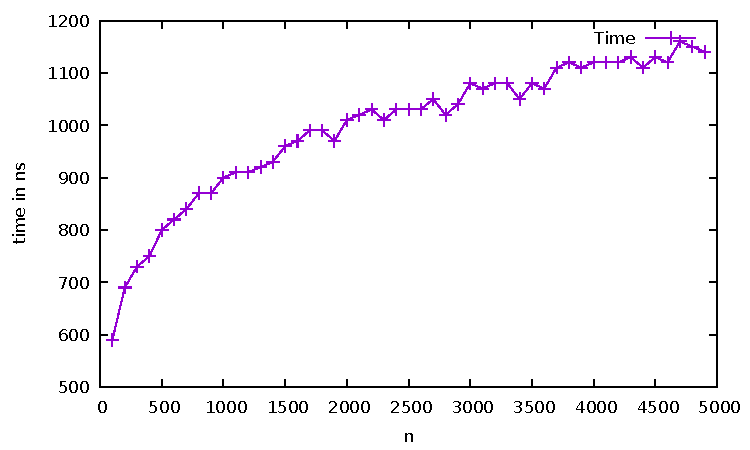
\includegraphics[width=\textwidth]{./binary_search/data} % Adjust width or height as needed
        \end{subfigure}
        \caption{Graph of binary searching through sorted arrays}
        \label{fig:graph_3}
    \end{figure}
    From the graph, we can clearly see that it is no longer a linear relationship.
    In fact this looks like a logarithmic time complexity.
    It is way more efficient than linear algorithms, allowing us to do operations on larger data sets.
    Running this algorithm on an array with 1 million items takes $570 ns$.
    This is a very huge boost compared to our linear algorithm.

    \section*{The cost of sorting}

    However, we cannot neglect the fact that we are working with sorted datasets.
    In real life, this is usually not the case, so we need to decide whether it is worth sorting the array first.
    The most efficient sorting algorithm (heapsort, merge sort, etc.) we know of has a time complexity of $O(n*log(n))$, which is quite expensive.

    It all depends on our use case: let's say we have a database where we store old cooking recipes.
    It means that we rarely update the database, but often read it.
    In this case, sorting our dataset could be worth it, since we do not have to do it regularly.
    On the other hand, when we are talking about a dataset that is frequently updated but barely read, sorting may not be worth it.

    \section*{Recursive binary search}

    Implementing binary search recursively is easier than most people think.
    We can simply remove the while loop and invoke the function where we used $continue$.
    Here is my implementation:

    \begin{minted}{c}
if (first == last) return false;
int mid = (first + last)/2;
if (array[mid] == key) return true;
if (array[mid] < key) {
    return binary_search(array, length, key, mid + 1, last);
} else {
    return binary_search(array, length, key, first, mid);
}
    \end{minted}

    Let's run the same benchmark as before, but utilizing our recursive function instead and compare the results.

    \begin{figure}[h]
        \centering
        \begin{subfigure}[b]{.5\textwidth}
            \centering
            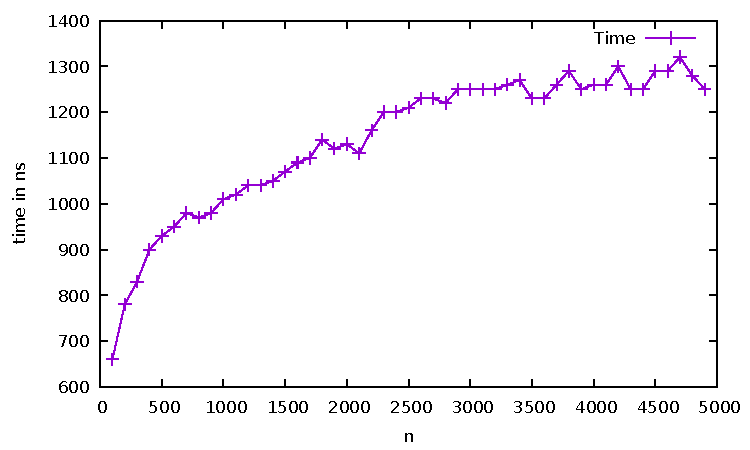
\includegraphics[width=\textwidth]{./binary_recursive/data} % Adjust width or height as needed
        \end{subfigure}
        \caption{Graph of recursive binary search}
        \label{fig:graph_4}
    \end{figure}

    We can see the logarithmic relationship here as well, but our runtime is actually slightly worse than before.
    The reason why it is slower is that procedure calls are more expensive.
    In this task, there is no clear reason to choose the recursive solution over the other, so let's just stick to the first one.

    \section*{GitHub}
    I have uploaded the full project to \underlinehref{https://github.com/peterherczku/ID1021/tree/main/assignment-3}{my github repository}, where you can find the code used to make this report.

\end{document}
